\documentclass[11pt,a4paper]{article}
\usepackage[utf8]{inputenc}
\usepackage[english]{babel}
\usepackage{amsmath}
\usepackage{amsfonts}
\usepackage{amssymb}
\usepackage{graphicx,float}
\usepackage{subcaption}
\usepackage{float}
\begin{document}
	\author{\textbf{Yaren Aksel}}
	\title{\textbf{Experiment 1, Stefan-Boltzmann Radiation Law}}
	\date{November 16, 2019}
	\maketitle
	\textit{with} {\large\textit{{Onuray Sancar}}\textit{,} \textit{Experiment Date}: November 8, 2019\\[2\baselineskip]
		\textbf{Abstract}\\[\baselineskip]
		\par In this experiment our aim is to observe the Stefann-Boltzmann law and inverse square law. To observing these relations we basically used a radiation sensor, a Stefan-Boltzmann lamp and a oven, with these heat sources and heat receiver by changing their inputs and distances between them we tried to observe these laws. For the square inverse law we found -1.321$\pm0.031$ and this value 22$\sigma$ away from -2. For the Stefann-Boltzmann law we found 2.17$\pm0.0831$ and this value 22$\sigma$ away from 4. These values seem to very far away from expected.
			\\[\baselineskip]
		\textbf{Theoretical Motivation}
		\\[\baselineskip]
		\par Since 1700s, natural philosophers knew that heat exchange between two bodies was not linearly dependent on the temperature difference. Even at high temperatures the discrepancy became greater. Over the years, many models were developed but none of them were as succesful as Josef Stefan's. He and a number of researchers with him proposed a unique relation to model the dependence of radiative heat exchange on the temperature in 1879. It was the $T^4$ law but Stefan's model was not widely accepted. Then, Stefan's former student Ludwig Boltzmann felt that there was some truth in the model proposed by his mentor. In 1884, Boltzmann showed that by treating electromagnetic radiation as the working fluid in a Carnot cycle the $T^4$ law was correct. The law applies only to blackbodies, theoretical surfaces that absord all incident heat radiation.$^{[1]}$
		\par The law can be derived from Planck's law by considering a small flat blackbody surface radiating out into a half-sphere.
		\begin{figure}[H]
			\begin{center}
				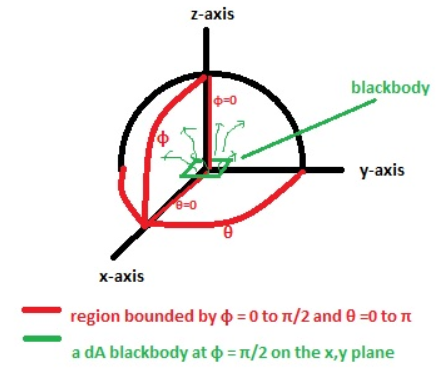
\includegraphics[scale=0.6]{pl.png}
			\end{center}
		\end{figure}
	    We can assume flat blackbody lies on the xy-plane. Using spherical coordinates and half-sphere boundaries we can derive the law.
	    \par The intensity of the light emitted from the blackbody surface is given by Planck's law:
	    \begin{equation}
	    I\left(\nu ,T\right)=\frac{2h{\nu }^{3}}{{c}^{2}}\frac{1}{{e}^{\frac{h\nu}{kT}}-1}
	    \end{equation}
	    where I($\nu$ ,T) is the amount of power per unit surface area per unit solid angle per unit frequency emitted at a frequency $\nu$ emitted by a black body at temperature T, h is Planck's constant, c is speed of light, k is Boltzmann's constant.\\
	    The quantity $I(\nu,T)Ad\nu d\Omega$ is the power radiated by a surface of area A through a solid angle $d\Omega$ in the frequency range between v and v+dv.\\
	    The Stefan-Boltzmann law gives the power emitted per unit area of the emitting body,
	    \begin{equation}
	    \frac{P}{A}=\underset{0}{\overset{\infty }{\int }}I\left(\nu ,T\right)d\nu \int \mathrm{cos}\theta d\Omega
	    \end{equation}
	    the cosine appears because black bodies are Lambertian meaning that the intensity observed along the sphere will be the actual intensity times the cosine of the zenith angle.
	    \begin{equation}
	    \frac{P}{A}=\underset{0}{\overset{\infty }{\int }}I\left(\nu ,T\right)d\nu \underset{0}{\overset{2\pi }{\int }}d\varphi \underset{0}{\overset{\pi/2}{\int }}{\mathrm{cos}}\theta \mathrm{sin}\theta d\theta \\= \pi\underset{0}{\overset{\infty }{\int }}I\left(\nu ,T\right)d\nu
	    \end{equation} 
	    To evaluate the integral, we can make a substitution,
	    \par $u=\frac{h\nu}{kT}$ and $du=\frac{h}{kT}d\nu$
	    \begin{equation}
	    \frac{P}{A}=\frac{2\pi h}{{c}^{2}}{\left(\frac{kT}{h}\right)}^{4}\underset{0}{\overset{\infty }{\int }}\frac{{u}^{3}}{{e}^{u}-1}du
	    \end{equation}
	    The integral in the right hand side of the equation is a very known integral and it gives the value $\frac {\pi^4}{15}$. Then, we get,$^{[2]}$
	    \begin{equation}
	    \frac{P}{A}=\sigma T^4, \sigma=\frac{2\pi^5k^4}{15c^2h^3}.
	    \end{equation}
	    For the calculation of error propagation we need the formula
	    \begin{equation}
	    {\sigma }_{f}=\sqrt{\sum _{i}^{n}{\left(\frac{\partial f}{\partial {x}_{i}}\right)}^{2}{\sigma }_{{x}_{i}}^{2}+\dots }
	    \end{equation}
	    Also, for the weighted average calculations we need
	    \begin{equation}
	    f_{weighted}=\frac{\sum _{i}\frac{{f}_{i}}{{\sigma_i }^{2}}}{\sum _{i}\frac{1}{{\sigma_i }^{2}}}
	    \end{equation}
	    where $\sigma_i$ is the uncertainty in $f_i$. \\[\baselineskip]
	    \textbf{Apparatus, Experimental Procedure, Data}
	    \\[\baselineskip] \textbf{\small{Apparatus}}(mainly)
	    \begin{itemize}
	    \item \textbf{Voltage Amplifier}: Because the received voltage is so low, we need to amplify it.
	    \item \textbf{Tungsten Lamp}: We used this as high temperature source.
	    \item \textbf{Radiation Sensor}: It converts received light into voltage.
	    \item \textbf{Ammeter}: We can give varying current to the set-up by this equipment.
	    \item \textbf{Voltmeter}: We can give varying voltage to the set-up by this equipment.
	    \item \textbf{Electrical Oven}: We used this as low temperature source.
	    \item \textbf{Temperature Probe with Display}: It is used to measure the temperature of the electrical oven.
	    \item \textbf{Ruler}: It is used to measure the distance between radiation sensor and tungsten lamp.
	    \item \textbf{Multimeters}: We measured more small values with these devices in some parts of the experiment.
	    \end{itemize}
    \textbf{\small{Procedure}}
    \begin{enumerate}
    	\item We connected sensor and tungsten lamp appropriately to the devices.
    	\item We adjusted the output voltage to give relevant values when we change scale of the voltage.
    	\item We connected multimeters to the set-up and then at 0-20mV applied voltage range we measured output voltage.
    	\item For the inverse square law part of the experiment: We first set the voltmeter to a value then by changing the distance between the sensor and the lamp we read the values on the voltage amplifier in the range of $3\times 10^{-2}$V and $10^{-3}$V.
    	\item For the high temperature part of the experiment: at the 3 different distances between the lamp and the sensor we took measurements for the varying current and voltage applied, output voltage.
    	\item For the low temperature part of the experiment: in this part we used the oven as radiation source. We placed sensor to the appropriate distance from the oven and also we placed a apparatus between them to reduce reflections. We collected data of temperature and output voltage as the temperature increase up to 400$^oC$.
    \end{enumerate}
        Some experimental conditions: The voltage amplifier doesn't make relevant measurements at high voltages. Measurements are done without measuring background radiation.
        \begin{figure}[H]
        	\begin{center}
        		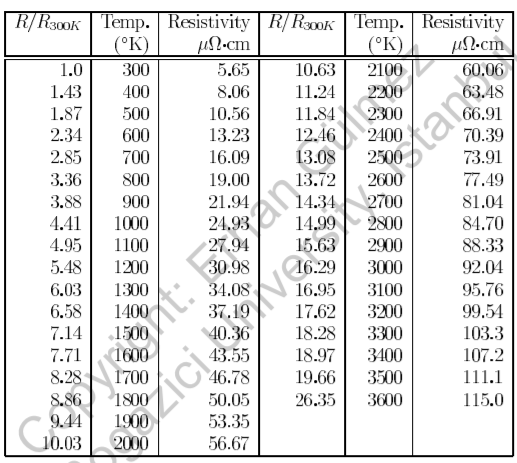
\includegraphics[scale=0.6]{R.png}
        	\end{center}
        \caption{Accepted values of R/$R_{300K}$ at different temperatures.}
        \end{figure} \newpage 
        \textbf{Analysis}\\[\baselineskip]
        \par We have done our data analysis using MATLAB. In MATLAB, one way to see the goodness of fit is to look at the R-square value. R-square always gives value between 0 and 1. Closer to 1 the R-square, the better the model fits data.
        \begin{figure}[H]
        	\begin{center}
        		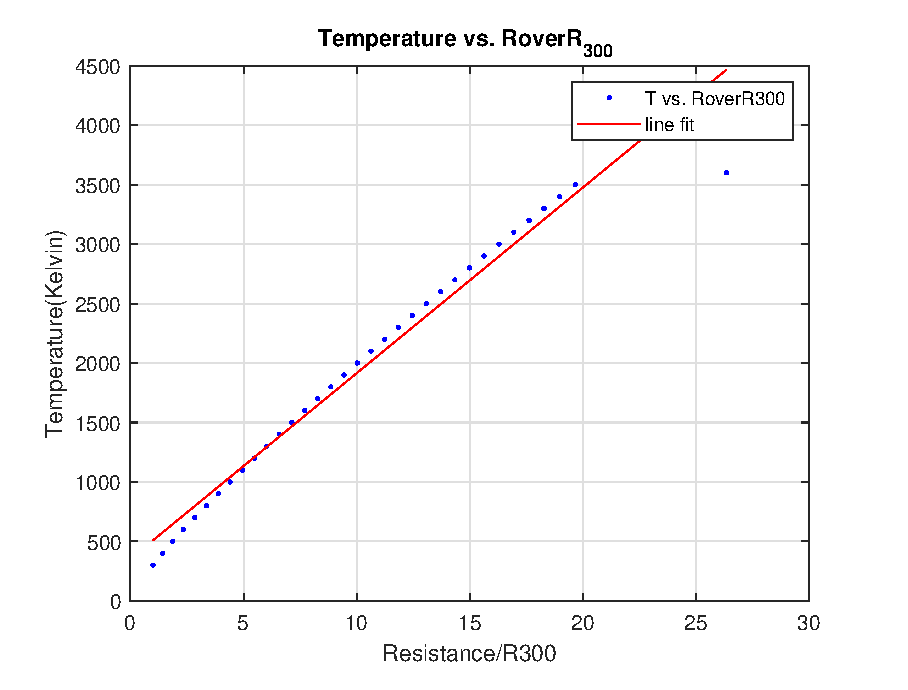
\includegraphics[scale=0.7]{RR.eps}
        	\end{center}
        	\caption{Fit function is  f(x) = p1*x + p2 with values: p1 =       145.1 $\pm0.8$, p2 =  351.5$\pm59.35$. R-square: 0.9701.}
        \end{figure}
    Here, we used table in the figure 1 to find R/$R_{300K}$ correspondence to the temperature. We fitted a line to temperature vs. R/$R_{300K}$ graph. This line-fit's information will be used in the upcoming parts of the analysis.
    \begin{figure}[H]
    	\begin{center}
    		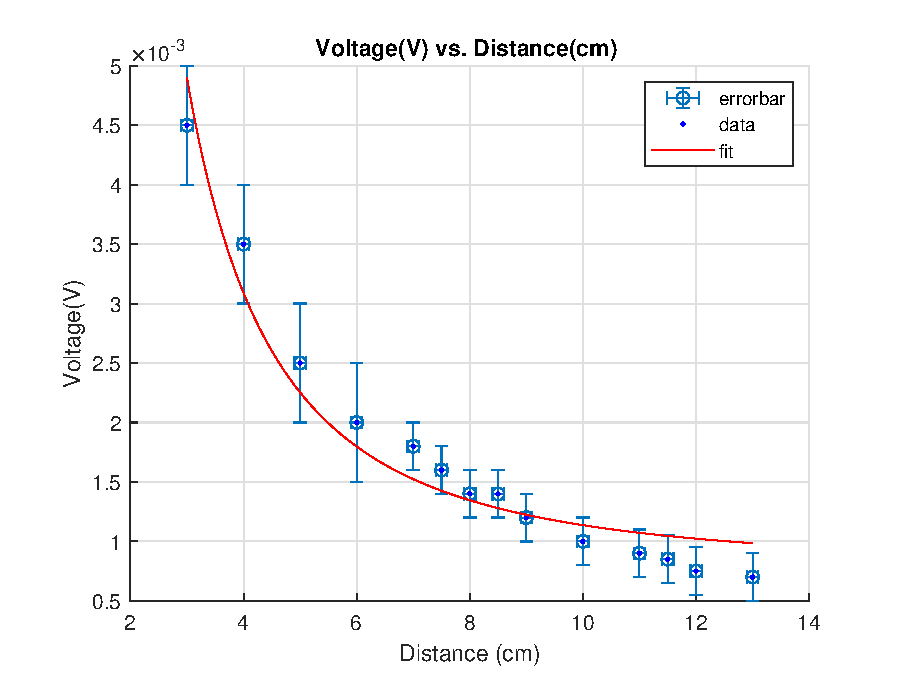
\includegraphics[scale=0.7]{inverse.eps}
    	\end{center}
    	\caption{Fit function is   f(x) = a*$x^{-2}$+b with values: a =      0.0402 $ \pm0.0072$ 
    		b =   0.0006765  $\pm0.0000711$ . R-square: 0.9574.}
    \end{figure}
\begin{figure}[H]
	\begin{center}
		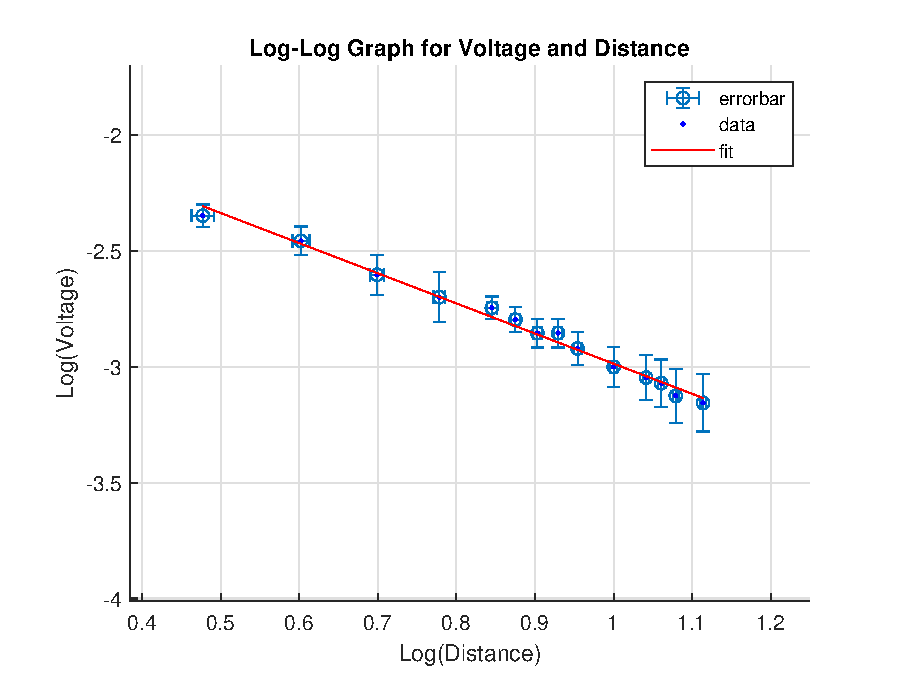
\includegraphics[scale=0.7]{inverselog.eps}
	\end{center}
	\caption{Fit function is  f(x) = p1*x + p2 with values: p1 =      -1.321 $\pm0.031$ 
		p2 =      -1.655 $\pm0.052$.R-square: 0.9904.}
\end{figure}
In this part of the analysis we fitted our datas first to a polynomial function. Then, we converted our datas to logarithms and we made a log-log graph. Making line-fit to the last graph helps us to easily see how voltage and distance relation changes in what power of a polynomial function. As we see voltage of the sensor decreases -1.321 power of the distance from the lamp. This is not near value to the -2 because it is $\frac{\left|-2+1.321\right|}{0,031}$=22$\sigma$ away from -2.
\begin{figure}[H]
	\begin{center}
		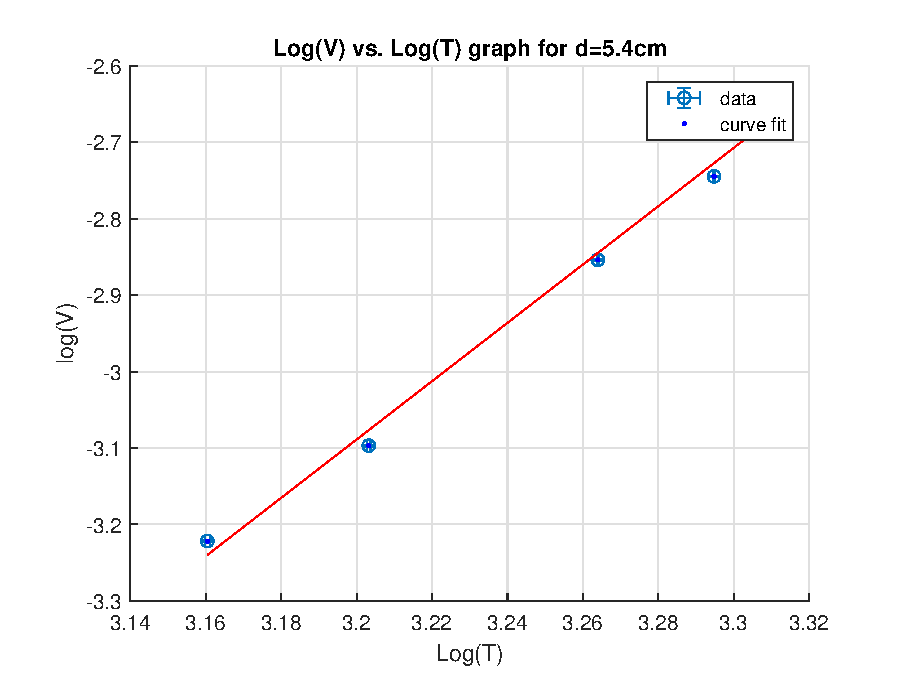
\includegraphics[scale=0.7]{d5.eps}
	\end{center}
	\caption{Fit function is f(x) = p1*x + p2 with values:  p1 =       5.786$\pm0.458$  
		p2 =       -20.2$ \pm 0.90$. R-square: 0.9935.}
\end{figure}
\begin{figure}[H]
	\begin{center}
		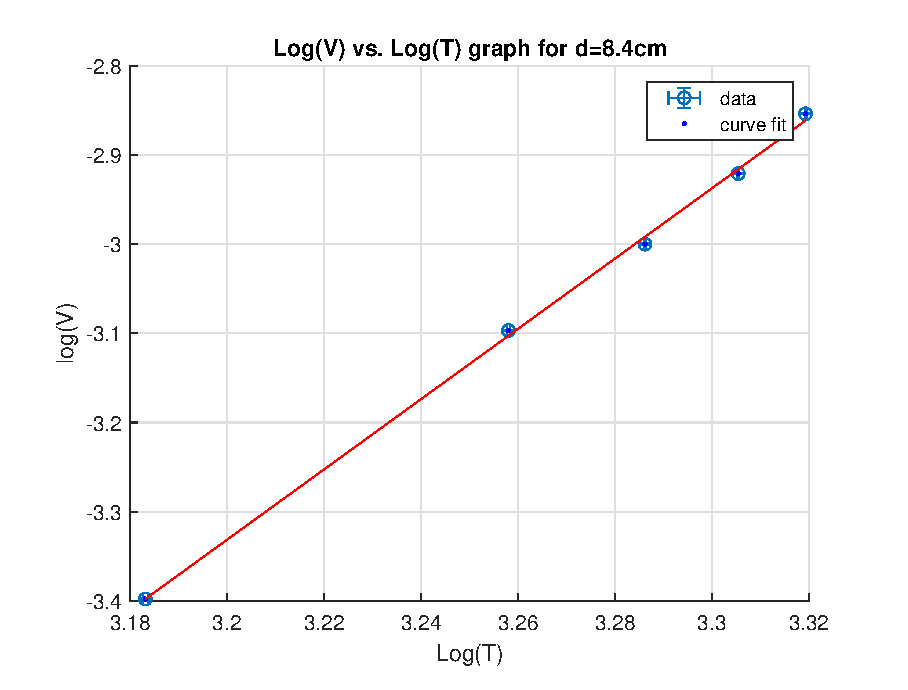
\includegraphics[scale=0.7]{d8.eps}
	\end{center}
	\caption{Fit function is f(x) = p1*x + p2 with values: p1 =       5.876 $\pm0.183$
		p2 =      -20.23 $\pm 0.42$. R-square: 0.997.}
\end{figure}
\begin{figure}[H]
	\begin{center}
		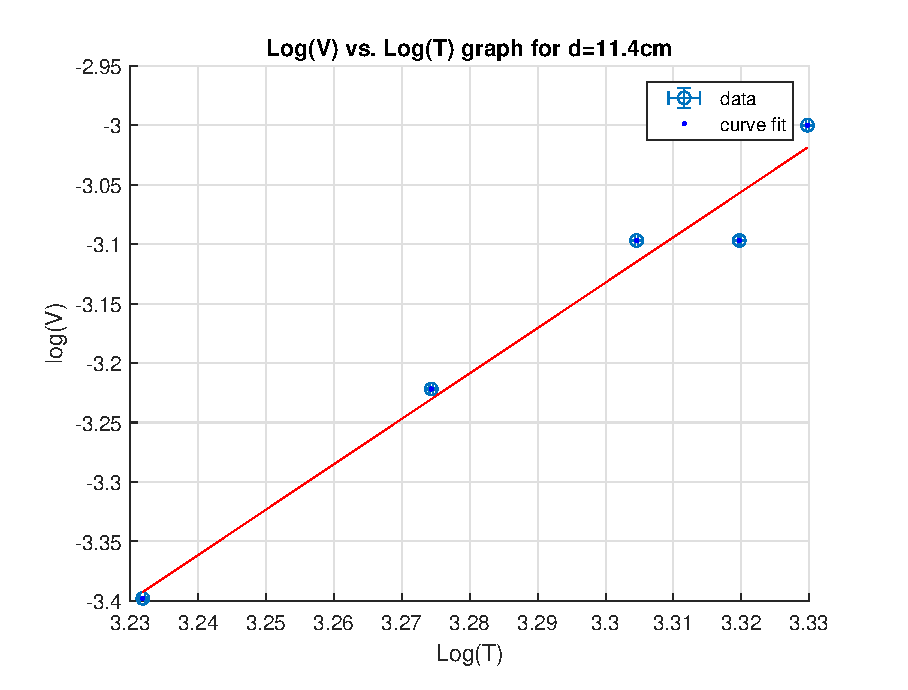
\includegraphics[scale=0.7]{d11.eps}
	\end{center}
	\caption{Fit function is f(x) = p1*x + p2 with values: p1 =       5.596$ \pm0.854$ 
			p2 =      -19.22 $\pm2.48$. R-square: 0.9750.}
\end{figure}
In the last three graphs our aim is to find received intensity of the radiation by the sensor is proportional to 4$^{th}$ power of temperature. As we said previously we see this kind of relations easily using log-log graphs. Now we have three p1s therefore it is a good idea to use equation (7) to get one weighted p1.
\begin{equation}
p1_{weighted}=\frac{\frac{5,786}{{\left(0,458\right)}^{2}}+\frac{5.876}{(0.183)^2}\frac{5.596}{(0.854)^2}}{\frac{1}{{\left(0.458\right)}^{2}}+\frac{1}{(0.183)^2}+\frac{1}{(0.854)^2}}=5.85\pm0.289
\end{equation}
The weighted value we found for p1 is 6.40$\sigma$ away from 4.
\begin{figure}[H]
	\begin{center}
		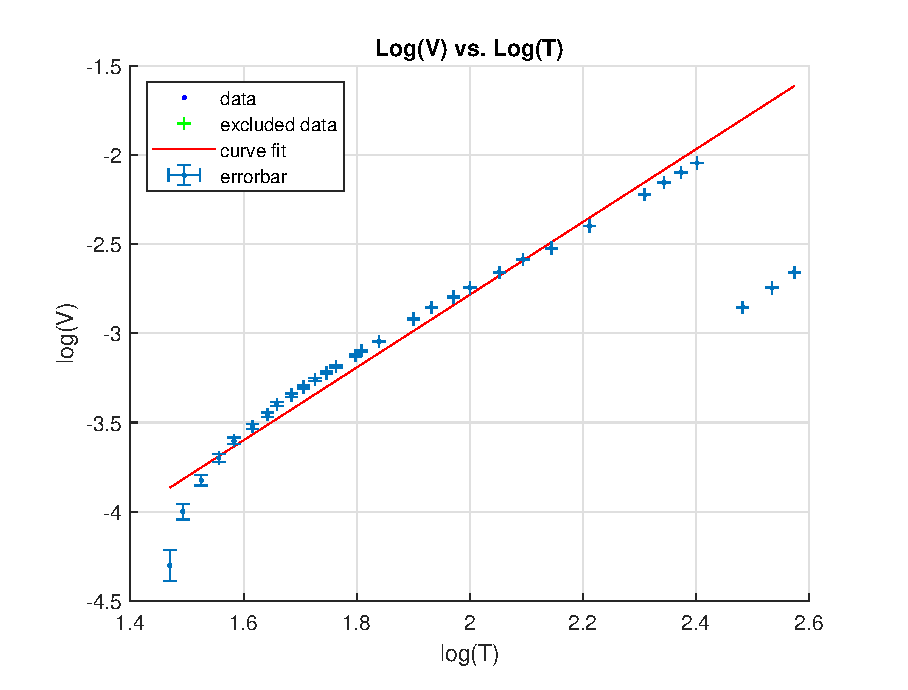
\includegraphics[scale=0.7]{low.eps}
	\end{center}
	\caption{Fit function is f(x) = p1*x + p2 with values:   p1 =        2.01 $\pm0.06$ 
		p2 =      -6.851$ \pm0.156$. R-square: 0.9657.}
\end{figure}
In the last graph of the analysis, again, we want to see T$^4$ law. In this part we made our experiment for low temperatures. Here we as we see from the curve fit our p1 is 2.01 $\pm0.06$.
\par Now, we can find from the last two p1s a final weighted p1:
\begin{equation}
p1_{weighted}=\frac{\frac{5,85}{{\left(0,289\right)}^{2}}+\frac{2.01}{(0.06)^2}}{\frac{1}{{\left(0.289\right)}^{2}}+\frac{1}{(0.06)^2}}=2.17\pm0.0831
\end{equation}
Our result for the p1 is 22.0$\sigma$ away from 4.\newpage 
\textbf{Conclusion}\\[\baselineskip]
\par As we see our n for T$^n$ is so far away from 4  but this is not a surprising result in the consideration of the errors we did during the experiment. Because we didn't act carefully some parts of the experiment. We sometimes leaned over to the lamp's side of the set-up and when we did that we didn't stop to taking data. This probably caused some changes in our datas. For the low temperature part of the experiment we didn't really examined the consistancy of the oven. Therefore, this may also be a cause of error. Also, we have done our experiment at the shiny surface of a table and we didn't make anything to prevent reflections from the table. The inverse square law part of the experiment didn't give a good result. The reasons of this are the same as stated for the other parts of the experiment. To improve these causes of errors we can isolate our set-up from the background radiation and radiation from humans. Also, buying a more advanced electric oven can improve the experiment.
	    \\[\baselineskip] \textbf{References}\\[\baselineskip]
		\par[1]A Brief History of the $T^4$ Radiation Law - Crepeau, John. \par https://pdfs.semanticscholar.org/748d/6a04e78f8dd3bdc15bdb74365e1a9db0667d.pdf 
		\par[2]Wikipedia, Stefan-Boltzmann Law.
		\par[3]Advanced Physics Experiments - Gülmez, Prof. Dr. Erhan.
		\\[\baselineskip] \textbf{Appendix}\\[\baselineskip]
		\textbf{\small{Raw Data}}
		\begin{center}
		\begin{figure} [H] 
			\begin{tabular}{|c |c||c|c|} \hline
				Potential Difference (mV)& Current (mA) & Potential Difference (mV)& Current (mA)\\ [0.5ex] 
				\hline
				0.8 & 2.75 & 9.2 &31.31\\
				\hline
				1.0 & 3.53 &9.9 & 33.73\\
				\hline 
				1.7 & 5.76 & 12.6 & 42.9\\
				\hline 
				2.3 & 7.40 & 14.5 & 49.4\\
				\hline 
				4.1 & 14.09 & 16.4 & 55.7\\
				\hline 
				5.5 & 18.66 & 17.8 & 6.4\\
				\hline 
				7.4 & 25.23 & 19.5 & 66.6\\
				\hline
			\end{tabular}
		\caption{Raw data for $0^{th}$ part of the experiment. Uncertainty of the potential differences is 0.1mV and uncertainty of the current is 0.01mA.}
	\end{figure}
\end{center}
\begin{center}
	\begin{figure} [H] 
		\begin{tabular}{|c |c||c|c|} \hline
			Potential Difference (V)& Distance (cm) & Potential Difference (V)& Distance (cm)\\ [0.5ex] 
			\hline
			0.45$\times10^{-2} \pm 0.05\times10^{-2}$ & 3.0$\pm0.1$ & 0.9$\times10^{-3} \pm 0.05\times10^{-3}$ &11.0$\pm0.1$\\
			\hline
			0.35$\times10^{-2} \pm 0.05\times10^{-2}$ & 4.0$\pm0.1$&0.85$\times10^{-3} \pm 0.05\times10^{-3}$ & 11.5$\pm0.1$\\
			\hline 
			0.25$\times10^{-2} \pm 0.05\times10^{-2}$ & 5.0$\pm0.1$ & 0.75$\times10^{-3} \pm 0.05\times10^{-3}$ &12.0$\pm0.1$\\
			\hline 
			0.20$\times10^{-2} \pm 0.05\times10^{-2}$ & 6.0$\pm0.1$ & 0.7$\times10^{-3} \pm 0.05\times10^{-3}$ & 13.0$\pm0.1$\\
			\hline 
			1.8$\times10^{-3} \pm 0.2\times10^{-3}$ & 7.0$\pm0.1$ &  & \\
			\hline 
			1.6$\times10^{-3} \pm 0.2\times10^{-3}$ & 7.5$\pm0.1$ &  &\\
			\hline 
			1.4$\times10^{-3} \pm 0.2\times10^{-3}$ & 8.0$\pm0.1$ &   & \\
			\hline
			1.4$\times10^{-3} \pm 0.2\times10^{-3}$&8.5$\pm0.1$& &\\
			\hline
			1.2$\times10^{-3} \pm 0.2\times10^{-3}$&9.0$\pm0.1$& &\\
			\hline
			1.0$\times10^{-3} \pm 0.2\times10^{-3}$&10.0$\pm0.1$& &\\
			\hline
		\end{tabular}
		\caption{Raw data for inverse square law part of the experiment with 0.9V of applied voltage and 2.3A of applied current.}
	\end{figure}
\end{center}
\begin{center}
	\begin{figure} [H] 
		\begin{tabular}{|c |c|c|} \hline
			Applied Potential Difference (V)& Applied Current(A) & Measured Potential Difference (V)\\ [0.5ex] 
			\hline
			6.77 & 2.232 & 1.8$\times10{-3}$\\
			\hline
			7.15 & 2.287 & 2.2$\times10{-3}$\\
			\hline
			5.60 & 2.015 & 1.4$\times10{-3}$\\
			\hline
			3.93 & 1.688 & 0.8$\times10{-3}$\\
			\hline
			3.088 & 1.509 & 0.6$\times10{-3}$\\
			\hline
		\end{tabular}
	\caption{Raw data for high temperature part of the experiment with distance between the lamp and the sensor 5.4$\pm0.1$cm. The uncertainty of applied voltages is 0.01V, the uncertainty of applied currents is 0.001A and the uncertainty of measured voltages is 0.0001V.}
\end{figure}
\end{center}
\begin{center}
	\begin{figure} [H] 
		\begin{tabular}{|c |c|c|} \hline
			Applied Potential Difference (V)& Applied Current(A) & Measured Potential Difference (V)\\ [0.5ex] 
			\hline
			3.511 & 1.601 & 0.4$\times10{-3}$\\
			\hline
			5.45 & 1.995 & 0.8$\times10{-3}$\\
			\hline
			6.40 & 2.162 & 1.0$\times10{-3}$\\
			\hline
			7.14 & 2.285 & 1.2$\times10{-3}$\\
			\hline
			7.75 & 2.386 & 1.4$\times10{-3}$\\
			\hline
		\end{tabular}
		\caption{Raw data for high temperature part of the experiment with distance between the lamp and the sensor 8.4$\pm0.1$cm. The uncertainty of applied voltages is 0.01V, the uncertainty of applied currents is 0.001A and the uncertainty of measured voltages is 0.0001V.}
	\end{figure}
\end{center}
\begin{center}
	\begin{figure} [H] 
		\begin{tabular}{|c |c|c|} \hline
			Applied Potential Difference (V)& Applied Current(A) & Measured Potential Difference (V)\\ [0.5ex] 
			\hline
			7.76 & 2.386 & 0.8$\times10{-3}$\\
			\hline
			7.09 & 2.274 & 0.8$\times10{-3}$\\
			\hline
			8.22 & 2.458 & 1.0$\times10{-3}$\\
			\hline
			5.94 & 2.075 & 0.6$\times10{-3}$\\
			\hline
			4.64 & 1.832 & 0.4$\times10{-3}$\\
			\hline
		\end{tabular}
		\caption{Raw data for high temperature part of the experiment with distance between the lamp and the sensor 11.4$\pm0.1$cm. The uncertainty of applied voltages is 0.01V, the uncertainty of applied currents is 0.001A and the uncertainty of measured voltages is 0.0001V.}
	\end{figure}
\end{center}
\begin{center}
	\begin{figure} [H] 
		\begin{tabular}{|c |c||c|c|} \hline
		    Temperature($^oC$)& Potential Difference(V) & Temperature($^oC$) & Potential Difference(V)\\ [0.5ex] 
			\hline
			29.5 $\pm0.1$ & 0.05$\times10{-3}$ & 79.5$\pm0.1$ &1.2$\times10{-3}$\\
			\hline
			31.1 $\pm0.1$ & 0.1$\times10{-3}$ &85.5$\pm0.1$ & 1.4$\times10{-3}$\\
			\hline 
			33.5 $\pm0.1$ & 0.15$\times10{-3}$ & 93.6$\pm0.1$ & 1.6$\times10{-3}$\\
			\hline 
			36.0  $\pm0.1$& 0.20$\times10{-3}$ & 100.0$\pm0.1$ &1.8$\times10{-3}$\\
			\hline 
			38.3$\pm0.1$ & 0.25$\times10{-3}$ & 112.8$\pm0.1$ & 2.2$\times10{-3}$\\
			\hline 
			41.3$\pm0.1$ & 0.30$\times10{-3}$ & 124.3$\pm0.1$ & 2.6$\times10{-3}$\\
			\hline 
			43.9$\pm0.1$ & 0.35$\times10{-3}$ & 139.4$\pm0.1$ & 3.0$\times10{-3}$\\
			\hline
			45.6$\pm0.1$ & 0.40$\times10{-3}$ & 162.7$\pm0.1$ & 4.0$\times10{-3}$\\
			\hline
			48.4$\pm0.1$ & 0.45$\times10{-3}$ & 203.7$\pm0.1$ & 6.0$\times10{-3}$\\
			\hline
			50.8$\pm0.1$ & 0.50$\times10{-3}$ & 220.4$\pm0.1$ & 7.0$\times10{-3}$\\
			\hline
			53.3$\pm0.1$ &0.55$\times10{-3}$ & 236.5$\pm0.1$  & 8.0$\times10{-3}$\\
			\hline
			55.8$\pm0.1$ &0.60$\times10{-3}$ & 252.3$\pm0.1$  & 9.0$\times10{-3}$\\
			\hline
			58.0$\pm0.1$ &0.65 $\times10{-3}$ & 303.6$\pm0.1$ & 14$\times10{-3}$\\
			\hline
			62.8$\pm0.1$ &0.75$\times10{-3}$ & 342.4$\pm0.1$  & 18$\times10{-3}$\\
			\hline
			64.4$\pm0.1$ &0.80$\times10{-3}$ & 374.8$\pm0.1$ &  22$\times10{-3}$\\
			\hline
			69.1$\pm0.1$ &0.90$\times10{-3}$ &        &             \\
			\hline
		\end{tabular}
		\caption{Raw data for low temperature part of the experiment.}
	\end{figure}
\begin{figure}[H]
	\begin{center}
		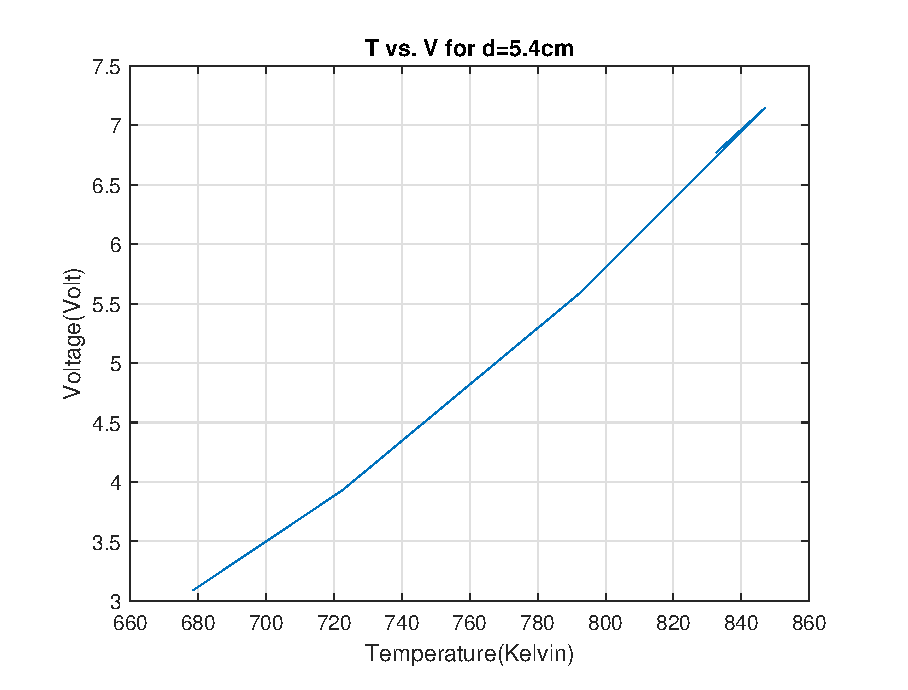
\includegraphics[scale=0.7]{5.eps}
	\end{center}
	\caption{Raw data graph of the high temperature part of the experiment.}
\end{figure}\begin{figure}[H]
\begin{center}
	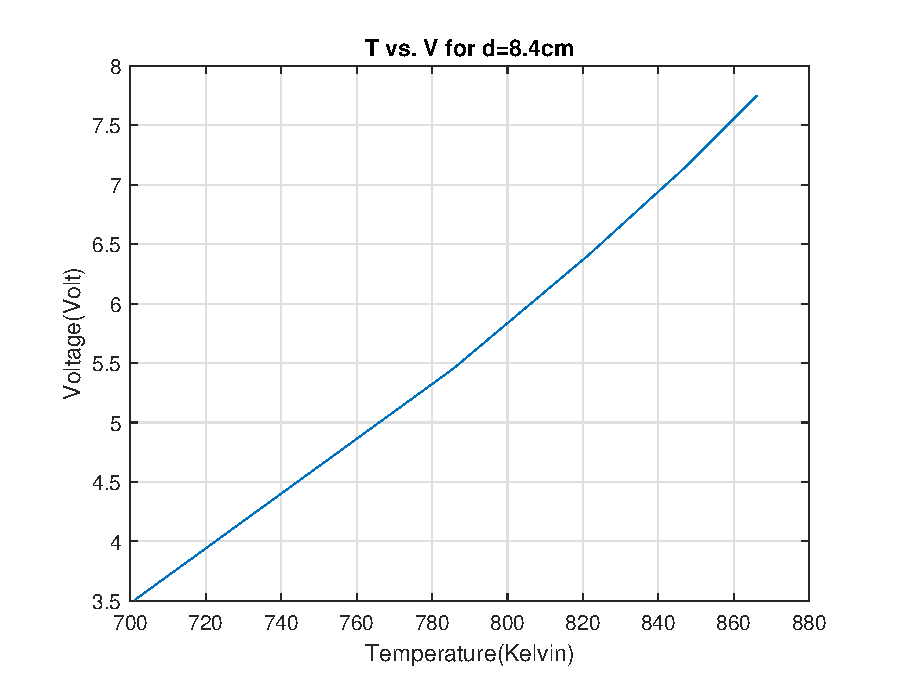
\includegraphics[scale=0.7]{8.eps}
\end{center}
\caption{Raw data graph of the high temperature part of the experiment.}
\end{figure}
\begin{figure}[H]
	\begin{center}
		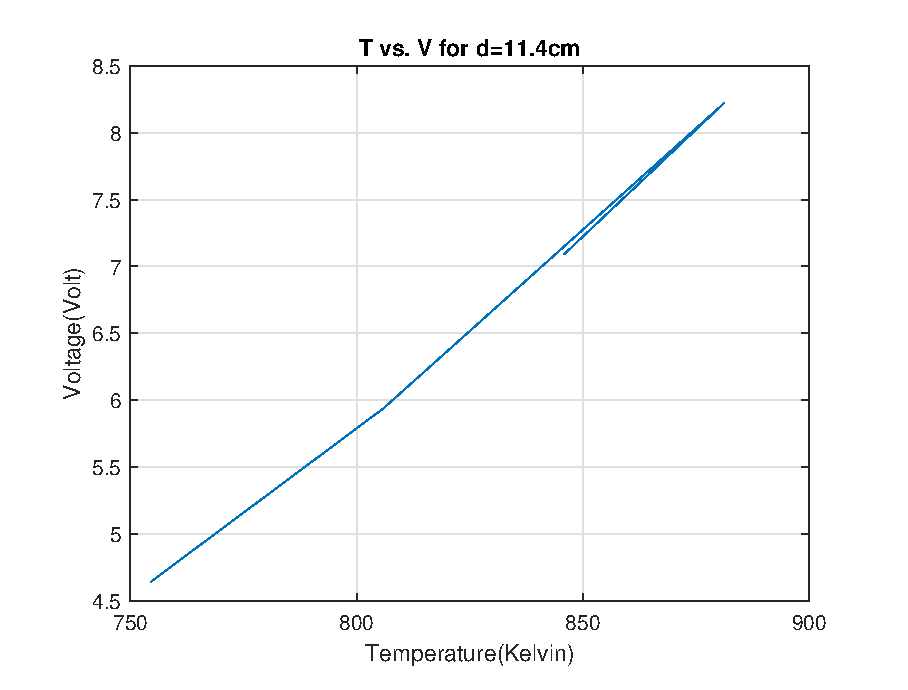
\includegraphics[scale=0.7]{11.eps}
	\end{center}
	\caption{Raw data graph of the high temperature part of the experiment.}
\end{figure}
\begin{figure}[H]
	\begin{center}
		\includegraphics[scale=0.7]{lowraw.eps}
	\end{center}
	\caption{Raw data graph of the low temperature part of the experiment.}
\end{figure}
\end{center}
\end{document}